\begin{figure}[H]
    \centering
    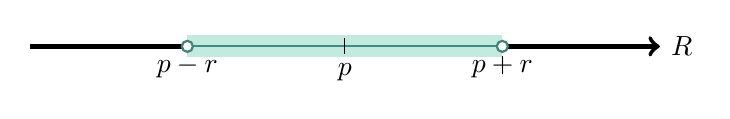
\begin{tikzpicture}
        % Eixo real.
        \draw[->,ultra thick] (-4,0)--(4,0) node[right]{$\mathbb R$};

        % Intervalo aberto ]p-r, p+r[.
        \draw[Emerald!24, line width=8pt] (-2,0) -- (2,0);
        \draw[Emerald!70!black, thick] (-2,0) -- (2,0);

        % Pontos abertos nas extremidades.
        \draw[fill=white, draw=Emerald!60!black, thick] (-2,0) circle (2pt) node[below]{$p - r$};
        \draw[fill=white, draw=Emerald!60!black, thick] (2,0) circle (2pt) node[below]{$p + r$};

        % Centro p.
        \draw (0,0.1) -- (0,-0.1) node[below]{$p$};
    \end{tikzpicture}
    \caption{Bola aberta de centro $p$ e raio $r$ em $\mathbb R$.}
    \label{fig:bolaAbertaR}
\end{figure}
